\documentclass{beamer}

\setbeamertemplate{footline}[frame number]

\usepackage{tikz}
\usepackage{centernot}
\usepackage[T1]{fontenc}


\title{Programmation système}
\author{Ordonnancement}
\date{loig.jezequel@univ-nantes.fr}

\begin{document}


\frame{
\maketitle
}

{
\setbeamertemplate{footline}{D'après A. Queudet \hfill \insertpagenumber\,/\,\inserttotalframenumber}

\frame{
\frametitle{Ordonnancement, schéma général}

\begin{block}{}
  L'ordonnancement consiste à \alert{choisir le processus/la tâche} à exécuter à chaque instant et \alert{déterminer le temps} durant lequel le processeur lui sera alloué.
\end{block}

\vspace*{0.5cm}

\scalebox{0.5}{
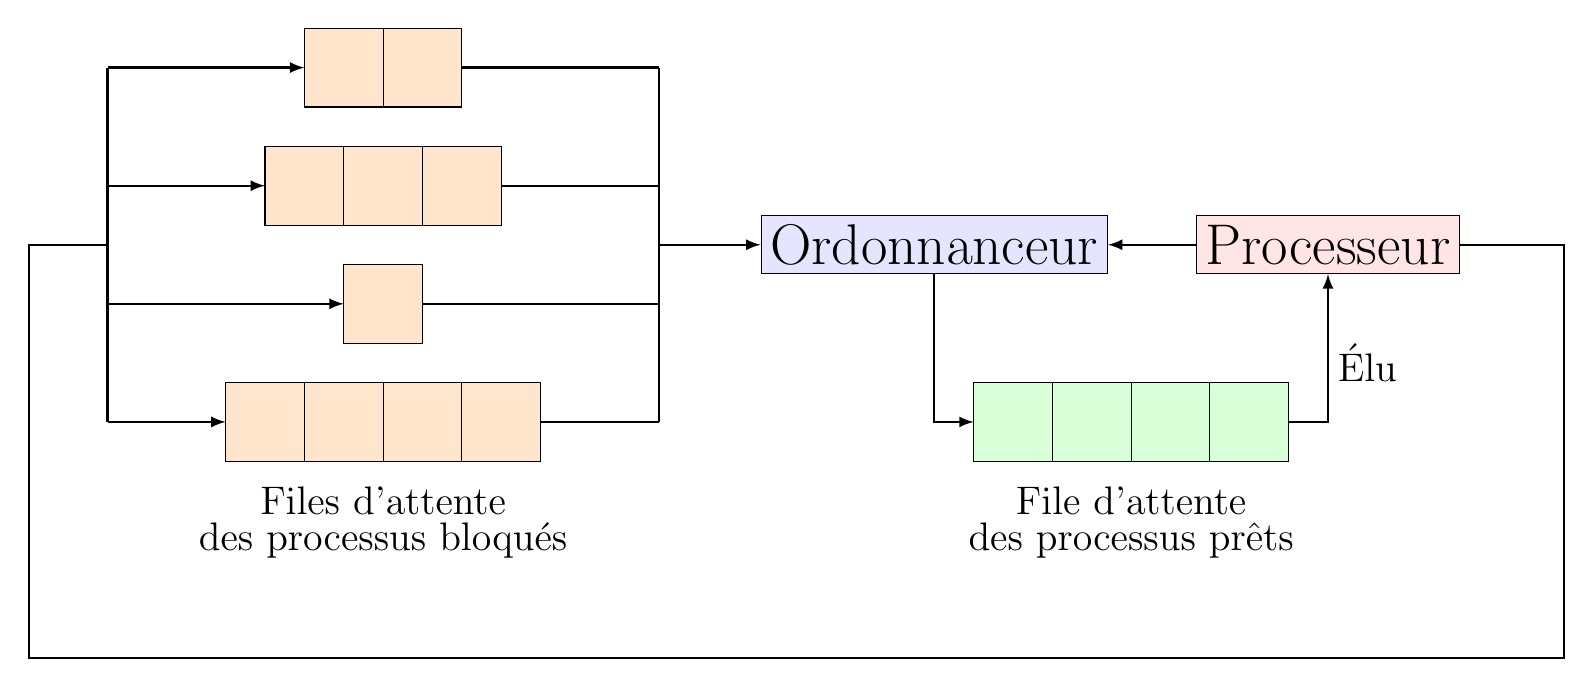
\begin{tikzpicture}

\draw[fill=orange!20] (0,0) rectangle (1,1);
\draw[fill=orange!20] (1,0) rectangle (2,1);
\draw[fill=orange!20] (2,0) rectangle (3,1);
\draw[fill=orange!20] (3,0) rectangle (4,1);

\draw[fill=orange!20] (1.5, 1.5) rectangle (2.5, 2.5);

\draw[fill=orange!20] (0.5, 3) rectangle (1.5, 4);
\draw[fill=orange!20] (1.5, 3) rectangle (2.5, 4);
\draw[fill=orange!20] (2.5, 3) rectangle (3.5, 4);

\draw[fill=orange!20] (1, 4.5) rectangle (2, 5.5);
\draw[fill=orange!20] (2, 4.5) rectangle (3, 5.5);

\node[rectangle,draw=black,fill=blue!10] (ord) at (9, 2.75) {\huge Ordonnanceur};

\node[rectangle,draw=black,fill=red!10] (proc) at (14, 2.75) {\huge Processeur};

\path[draw=black,thick] (3, 5) -- (5.5, 5);
\path[draw=black,thick] (3.5, 3.5) -- (5.5, 3.5);
\path[draw=black,thick] (2.5, 2) -- (5.5, 2);
\path[draw=black,thick] (4, 0.5) -- (5.5, 0.5);
\path[draw=black,thick] (5.5, 5) -- (5.5, 0.5);
\path[draw=black,-latex,thick] (5.5, 2.75) -- (ord);
\path[draw=black,-latex,thick] (proc) -- (ord);

\draw[fill=green!15] (9.5,0) rectangle (10.5,1);
\draw[fill=green!15] (10.5,0) rectangle (11.5,1);
\draw[fill=green!15] (11.5,0) rectangle (12.5,1);
\draw[fill=green!15] (12.5,0) rectangle (13.5,1);

\path[draw=black,-latex,thick] (ord) -- (9, 0.5) -- (9.5, 0.5);
\path[draw=black,-latex,thick] (13.5, 0.5) -- (14, 0.5) -- (proc);

\path[draw=black,thick] (proc) -- (17, 2.75) -- (17, -2.5) -- (-2.5, -2.5) -- (-2.5, 2.75) -- (-1.5, 2.75);

\path[draw=black,-latex,thick] (-1.5, 5) -- (1, 5);
\path[draw=black,-latex,thick] (-1.5, 3.5) -- (0.5, 3.5);
\path[draw=black,-latex,thick] (-1.5, 2) -- (1.5, 2);
\path[draw=black,-latex,thick] (-1.5, 0.5) -- (0, 0.5);
\path[draw=black,thick] (-1.5, 5) -- (-1.5, 0.5);

\node (info) at (2, -0.5) {\Large Files d'attente};
\node (info) at (2, -1) {\Large des processus bloqués};

\node (info) at (11.5, -0.5) {\Large File d'attente};
\node (info) at (11.5, -1) {\Large des processus prêts};

\node (info) at (14.5, 1.25) {\Large Élu};
\end{tikzpicture}
}

\begin{block}{}
L'\alert{ordonnanceur} alloue le processeur aux différents processus selon un \alert{algorithme d'ordonnancement} donné.
\end{block}

}

\frame{
\frametitle{Objectifs de l'ordonnancement}

\begin{block}{Approche naïve}
On pourrait juste exécuter les processus quand ils arrivent (premier arrivé premier servi)
\end{block}

\begin{block}{Objectifs de l'ordonnancement}
\begin{itemize}
\item Minimiser le nombre de changements de contexte
\item Maximiser le nombre de processus exécutés par unité de temps
\item Minimiser le temps d'attente de chaque processus
\item Maximiser le temps d'utilisation des processeurs
\item Favoriser les processus prioritaire
\end{itemize}
\end{block}

}

\frame{
\frametitle{Types d'algorithmes d'ordonnancement}

\begin{itemize}
\item Monoprocesseur/multiprocesseur
\begin{itemize}
\item ordonnancer les processus sur un ou plusieurs processeurs ne se fait pas de la même façon
\end{itemize}
\item En ligne/Hors ligne
\begin{itemize}
\item les processus peuvent être ordonnancés une fois pour toute ou bien au fur et à mesure de leur création
\end{itemize}
\item Préemptif/Non préemptif
\begin{itemize}
\item on peut parfois interrompre un processus en cours à la demande de l'ordonnanceur
\end{itemize}
\item Oisif/Non oisif
\begin{itemize}
\item un processeur peut parfois être laissé inactif alors que des processus sont en attente d'être exécutés
\end{itemize}
\item Centralisé/Réparti
\end{itemize}

}

\frame{
\frametitle{Méthodes classiques d'ordonnancement}

\begin{block}{Non préemptif}
\begin{itemize}
\item Selon l'ordre d'arrivée\\ \hspace{1cm} (First Come First Served, FCFS)
\item Selon la durée de calcul\\ \hspace{1cm} (Shortest Job First, SJF)
\end{itemize}
\end{block}

\begin{block}{Préemptif}
\begin{itemize}
\item Selon la durée de calcul restante\\ \hspace{1cm} (Shortest Remaining Time, SRT)
\item Temps partagé avec politique du tourniquet\\ \hspace{1cm} (Round-Robin, RR)
\item Selon la priorité des tâches
\end{itemize}
\end{block}

}

\frame{
\frametitle{Ordonnancement First Come First Served}

\begin{block}{Principe}
Les tâches sont ordonnancées selon leur ordre d'arrivée
\end{block}

\begin{exampleblock}{Exemple}
  $P_1$ (arrive à $t=0$, durée 53), $P_2$ (à $t=10$, durée 17), $P_3$ (à $t=20$, durée 68), $P_4$ (à $t=30$, durée 24)
\end{exampleblock}

\begin{center}
\scalebox{0.8}{
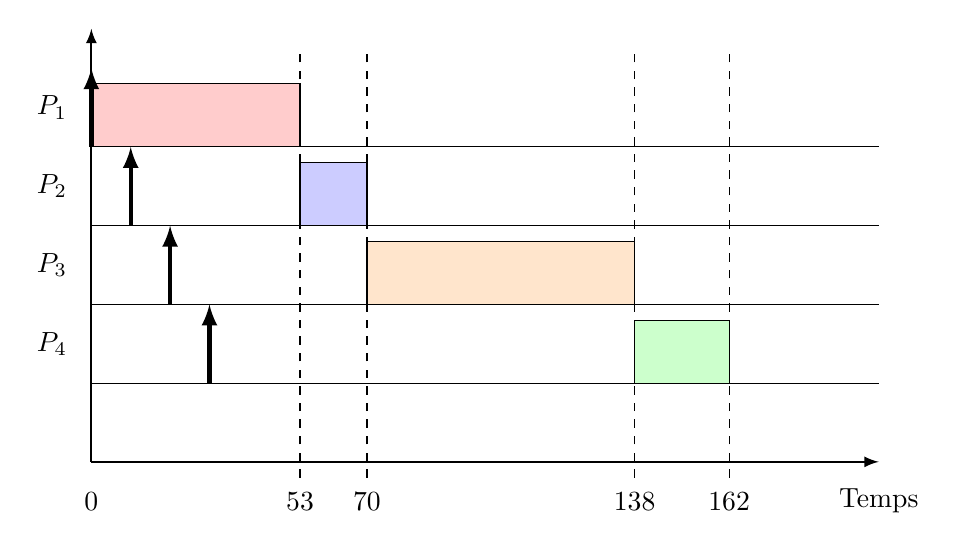
\begin{tikzpicture}

\path[draw=black,-latex,thick] (0,0) -- (0,5.5);
\path[draw=black,-latex,thick] (0,0) -- (10,0);

\path[draw=black] (0,1) -- (10,1);
\path[draw=black] (0,2) -- (10,2);
\path[draw=black] (0,3) -- (10,3);
\path[draw=black] (0,4) -- (10,4);

\node (t) at (0,-0.5) {0};
\node (t) at (10,-0.5) {Temps};

\path[draw=black,dashed] (2.65,-0.2) -- (2.65,5.2);
\node (t) at (2.65,-0.5) {53};
\path[draw=black,dashed] (3.5,-0.2) -- (3.5,5.2);
\node (t) at (3.5,-0.5) {70};
\path[draw=black,dashed] (6.9,-0.2) -- (6.9,5.2);
\node (t) at (6.9,-0.5) {138};
\path[draw=black,dashed] (8.1,-0.2) -- (8.1,5.2);
\node (t) at (8.1,-0.5) {162};

%p1
\node (p1) at (-0.5,4.5) {$P_1$};
\draw[draw=black,fill=red!20] (0,4) rectangle (2.65,4.8);
\path[draw=black,-latex,ultra thick] (0,4) -- (0,5);

%p2
\node (p2) at (-0.5,3.5) {$P_2$};
\draw[draw=black,fill=blue!20] (2.65,3) rectangle (3.5,3.8);
\path[draw=black,-latex,ultra thick] (0.5,3) -- (0.5,4);

%p3
\node (p3) at (-0.5,2.5) {$P_3$};
\draw[draw=black,fill=orange!20] (3.5,2) rectangle (6.9,2.8);
\path[draw=black,-latex,ultra thick] (1,2) -- (1,3);

%p4
\node (p4) at (-0.5,1.5) {$P_4$};
\draw[draw=black,fill=green!20] (6.9,1) rectangle (8.1,1.8);
\path[draw=black,-latex,ultra thick] (1.5,1) -- (1.5,2);

\end{tikzpicture}
}
\end{center}

}

\frame{
\frametitle{Ordonnancement First Come First Served, suite}

\begin{block}{Avantages}
\begin{itemize}
\item Faible complexité d'implantation (simplement basé sur une file)
\end{itemize}
\end{block}

\begin{block}{Inconvénients}
\begin{itemize}
\item Pas de prise en compte de l'importance relative des tâches
\item Temps d'attente du processeur par les tâches généralement important
\end{itemize}
\end{block}

}

\frame{
\frametitle{Ordonnancement Shortest Job First}

\begin{block}{Principe}
La tâche dont le temps d'exécution est le plus court est ordonnancée en priorité
\end{block}

\begin{exampleblock}{Exemple}
  $P_1$ (arrive à $t=0$, durée 53), $P_2$ (à $t=0$, durée 17), $P_3$ (à $t=0$, durée 68), $P_4$ (à $t=0$, durée 24)
\end{exampleblock}

\only<1>{\vspace*{1cm}\centering \alert{Représentez l'histogramme de l'exécution des tâches\\ par le processeur}}


\pause

\begin{center}
\scalebox{0.8}{
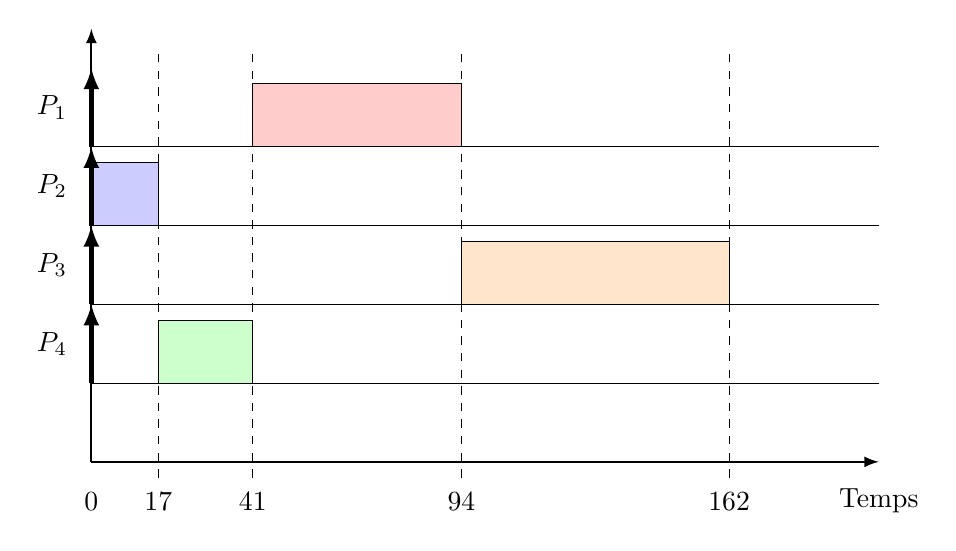
\begin{tikzpicture}

\path[draw=black,-latex,thick] (0,0) -- (0,5.5);
\path[draw=black,-latex,thick] (0,0) -- (10,0);

\path[draw=black] (0,1) -- (10,1);
\path[draw=black] (0,2) -- (10,2);
\path[draw=black] (0,3) -- (10,3);
\path[draw=black] (0,4) -- (10,4);

\node (t) at (0,-0.5) {0};
\node (t) at (10,-0.5) {Temps};

\path[draw=black,dashed] (0.85,-0.2) -- (0.85,5.2);
\node (t) at (0.85,-0.5) {17};
\path[draw=black,dashed] (2.05,-0.2) -- (2.05,5.2);
\node (t) at (2.05,-0.5) {41};
\path[draw=black,dashed] (4.7,-0.2) -- (4.7,5.2);
\node (t) at (4.7,-0.5) {94};
\path[draw=black,dashed] (8.1,-0.2) -- (8.1,5.2);
\node (t) at (8.1,-0.5) {162};

%p1
\node (p1) at (-0.5,4.5) {$P_1$};
\draw[draw=black,fill=red!20] (2.05,4) rectangle (4.7,4.8);
\path[draw=black,-latex,ultra thick] (0,4) -- (0,5);

%p2
\node (p2) at (-0.5,3.5) {$P_2$};
\draw[draw=black,fill=blue!20] (0,3) rectangle (0.85,3.8);
\path[draw=black,-latex,ultra thick] (0,3) -- (0,4);

%p3
\node (p3) at (-0.5,2.5) {$P_3$};
\draw[draw=black,fill=orange!20] (4.7,2) rectangle (8.1,2.8);
\path[draw=black,-latex,ultra thick] (0,2) -- (0,3);

%p4
\node (p4) at (-0.5,1.5) {$P_4$};
\draw[draw=black,fill=green!20] (0.85,1) rectangle (2.05,1.8);
\path[draw=black,-latex,ultra thick] (0,1) -- (0,2);

\end{tikzpicture}
}
\end{center}

}

\frame{
\frametitle{Ordonnancement Shortest Job First, suite}

\begin{block}{Avantages}
\begin{itemize}
\item Réduit le temps d'attente des processus (par rapport à FCFS)
\end{itemize}
\end{block}

\begin{block}{Inconvénients}
\begin{itemize}
\item Pas de prise en compte de l'importance relative des tâches
\item Optimal seulement si tous les processus sont disponibles simultanément
\end{itemize}
\end{block}

}


\frame{
\frametitle{Ordonnancement Shortest Remaining Time}

\begin{block}{Principe}
La tâche dont le temps d'exécution restant est le plus court parmi celles qui restent à exécuter est ordonnancée en premier
\end{block}

\begin{exampleblock}{Exemple}
  $P_1$ (arrive à $t=50$, durée 53), $P_2$ (à $t=20$, durée 17), $P_3$ (à $t=0$, durée 68), $P_4$ (à $t=0$, durée 24)
\end{exampleblock}

\only<1>{\vspace*{1cm}\centering \alert{Représentez l'histogramme de l'exécution des tâches\\ par le processeur}}


\pause

\begin{center}
\scalebox{0.8}{
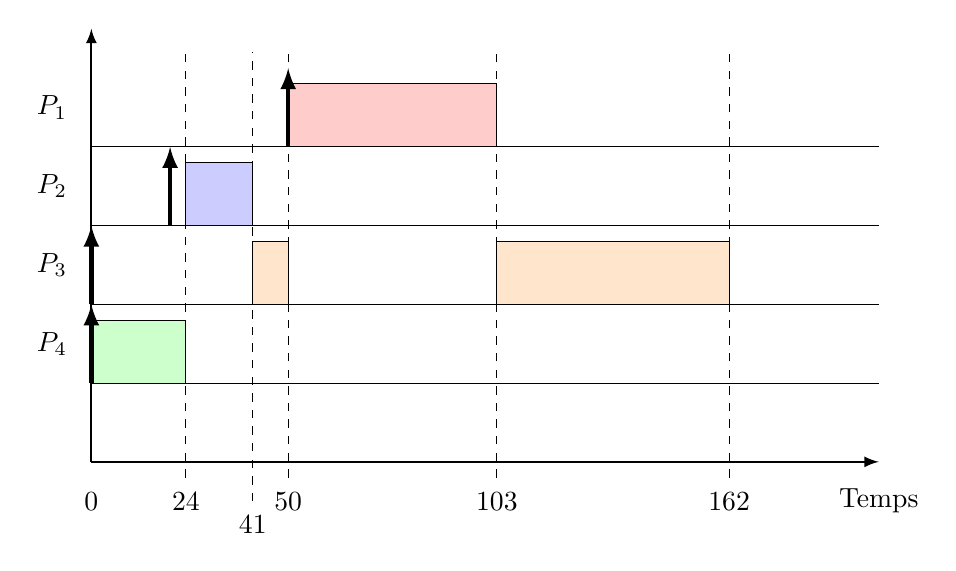
\begin{tikzpicture}

\path[draw=black,-latex,thick] (0,0) -- (0,5.5);
\path[draw=black,-latex,thick] (0,0) -- (10,0);

\path[draw=black] (0,1) -- (10,1);
\path[draw=black] (0,2) -- (10,2);
\path[draw=black] (0,3) -- (10,3);
\path[draw=black] (0,4) -- (10,4);

\node (t) at (0,-0.5) {0};
\node (t) at (10,-0.5) {Temps};

\path[draw=black,dashed] (1.2,-0.2) -- (1.2,5.2);
\node (t) at (1.2,-0.5) {24};
\path[draw=black,dashed] (2.05,-0.5) -- (2.05,5.2);
\node (t) at (2.05,-0.8) {41};
\path[draw=black,dashed] (2.5,-0.2) -- (2.5,5.2);
\node (t) at (2.5,-0.5) {50};
\path[draw=black,dashed] (5.15,-0.2) -- (5.15,5.2);
\node (t) at (5.15,-0.5) {103};
\path[draw=black,dashed] (8.1,-0.2) -- (8.1,5.2);
\node (t) at (8.1,-0.5) {162};

%p1
\node (p1) at (-0.5,4.5) {$P_1$};
\draw[draw=black,fill=red!20] (2.5,4) rectangle (5.15,4.8);
\path[draw=black,-latex,ultra thick] (2.5,4) -- (2.5,5);

%p2
\node (p2) at (-0.5,3.5) {$P_2$};
\draw[draw=black,fill=blue!20] (1.2,3) rectangle (2.05,3.8);
\path[draw=black,-latex,ultra thick] (1,3) -- (1,4);

%p3
\node (p3) at (-0.5,2.5) {$P_3$};
\draw[draw=black,fill=orange!20] (2.05,2) rectangle (2.5,2.8);
\draw[draw=black,fill=orange!20] (5.15,2) rectangle (8.1,2.8);
\path[draw=black,-latex,ultra thick] (0,2) -- (0,3);

%p4
\node (p4) at (-0.5,1.5) {$P_4$};
\draw[draw=black,fill=green!20] (0,1) rectangle (1.2,1.8);
\path[draw=black,-latex,ultra thick] (0,1) -- (0,2);

\end{tikzpicture}
}
\end{center}

}

\frame{
\frametitle{Ordonnancement Shortest Remaining Time, suite}

\begin{block}{Avantages}
\begin{itemize}
\item Minimise le temps d'attente moyen des processus courts
\end{itemize}
\end{block}

\begin{block}{Inconvénients}
\begin{itemize}
\item Pas de prise en compte de l'importance relative des tâches
\item Non équité de service~: les processus longs sont pénalisés
\item Possibilité de famine pour les processus les plus longs
\end{itemize}
\end{block}

}

\frame{
\frametitle{Ordonnancement Round Robin}

\begin{block}{Principe}
Le processeur est alloué par tranches de temps de taille fixe (quantum), chacun son tour.
\end{block}

\begin{exampleblock}{Exemple}
  $P_1$ (arrive à $t=0$, durée 53), $P_2$ (à $t=0$, durée 17), $P_3$ (à $t=0$, durée 68), $P_4$ (à $t=0$, durée 24), le quantum vaut 20
\end{exampleblock}

\only<1>{\vspace*{1cm}\centering \alert{Représentez l'histogramme de l'exécution des tâches\\ par le processeur}}


\pause

\begin{center}
\scalebox{0.8}{
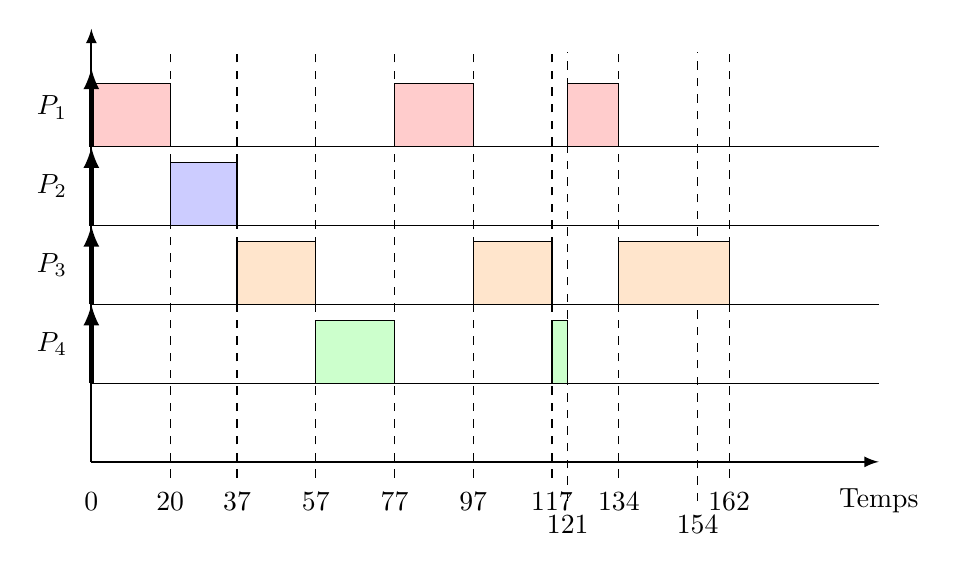
\begin{tikzpicture}

\path[draw=black,-latex,thick] (0,0) -- (0,5.5);
\path[draw=black,-latex,thick] (0,0) -- (10,0);

\path[draw=black] (0,1) -- (10,1);
\path[draw=black] (0,2) -- (10,2);
\path[draw=black] (0,3) -- (10,3);
\path[draw=black] (0,4) -- (10,4);

\node (t) at (0,-0.5) {0};
\node (t) at (10,-0.5) {Temps};

\path[draw=black,dashed] (1,-0.2) -- (1,5.2);
\node (t) at (1,-0.5) {20};
\path[draw=black,dashed] (1.85,-0.2) -- (1.85,5.2);
\node (t) at (1.85,-0.5) {37};
\path[draw=black,dashed] (2.85,-0.2) -- (2.85,5.2);
\node (t) at (2.85,-0.5) {57};
\path[draw=black,dashed] (3.85,-0.2) -- (3.85,5.2);
\node (t) at (3.85,-0.5) {77};
\path[draw=black,dashed] (4.85,-0.2) -- (4.85,5.2);
\node (t) at (4.85,-0.5) {97};
\path[draw=black,dashed] (5.85,-0.2) -- (5.85,5.2);
\node (t) at (5.85,-0.5) {117};
\path[draw=black,dashed] (6.05,-0.5) -- (6.05,5.2);
\node (t) at (6.05,-0.8) {121};
\path[draw=black,dashed] (6.7,-0.2) -- (6.7,5.2);
\node (t) at (6.7,-0.5) {134};
\path[draw=black,dashed] (7.7,-0.5) -- (7.7,5.2);
\node (t) at (7.7,-0.8) {154};
\path[draw=black,dashed] (8.1,-0.2) -- (8.1,5.2);
\node (t) at (8.1,-0.5) {162};

%p1
\node (p1) at (-0.5,4.5) {$P_1$};
\draw[draw=black,fill=red!20] (0,4) rectangle (1,4.8);
\draw[draw=black,fill=red!20] (3.85,4) rectangle (4.85,4.8);
\draw[draw=black,fill=red!20] (6.05,4) rectangle (6.7,4.8);
\path[draw=black,-latex,ultra thick] (0,4) -- (0,5);

%p2
\node (p2) at (-0.5,3.5) {$P_2$};
\draw[draw=black,fill=blue!20] (1,3) rectangle (1.85,3.8);
\path[draw=black,-latex,ultra thick] (0,3) -- (0,4);

%p3
\node (p3) at (-0.5,2.5) {$P_3$};
\draw[draw=black,fill=orange!20] (1.85,2) rectangle (2.85,2.8);
\draw[draw=black,fill=orange!20] (4.85,2) rectangle (5.85,2.8);
\draw[draw=black,fill=orange!20] (6.7,2) rectangle (8.1,2.8);
\path[draw=black,-latex,ultra thick] (0,2) -- (0,3);

%p4
\node (p4) at (-0.5,1.5) {$P_4$};
\draw[draw=black,fill=green!20] (2.85,1) rectangle (3.85,1.8);
\draw[draw=black,fill=green!20] (5.85,1) rectangle (6.05,1.8);
\path[draw=black,-latex,ultra thick] (0,1) -- (0,2);

\end{tikzpicture}
}
\end{center}

}

\frame{
\frametitle{Ordonnancement Round Robin, suite}

\begin{block}{Avantages}
\begin{itemize}
\item Équité de l'attribution du processeur entre toutes les tâches
\item Avec $n$ tâches, chacune obtient le processeur au bout de $(n-1)\times q$ unités de temps au maximum
\end{itemize}
\end{block}

\begin{block}{Inconvénients}
\begin{itemize}
\item Pas de prise en compte de l'importance relative des tâches
\item Difficulté du choix de la tranche de temps
\begin{itemize}
\item trop grande, Round Robin équivalent à FCFS
\item trop petite, beaucoup de changements de contexte
\end{itemize}
\end{itemize}
\end{block}

}

\frame{
\frametitle{Ordonnancement à priorités statiques}

\begin{block}{Principe}
Le processeur est alloué selon des priorités affectées aux tâches pour toute la durée de vie de l'application
\end{block}

\begin{exampleblock}{Exemple}
  $P_1$ (à $t=0$, $d=53$, priorité 0), $P_2$ (à $t=0$, $d=17$, priorité 1), $P_3$ (à $t=0$, $d=68$, priorité 3), $P_4$ (à $t=0$, $d=24$, priorité 2)
\end{exampleblock}

\only<1>{\vspace*{1cm}\centering \alert{Représentez l'histogramme de l'exécution des tâches\\ par le processeur}}


\pause

\begin{center}
\scalebox{0.8}{
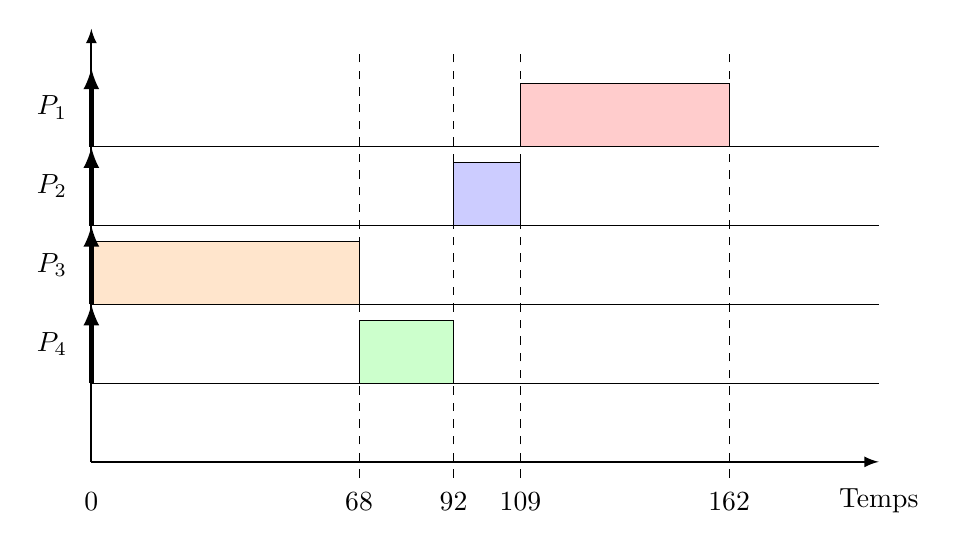
\begin{tikzpicture}

\path[draw=black,-latex,thick] (0,0) -- (0,5.5);
\path[draw=black,-latex,thick] (0,0) -- (10,0);

\path[draw=black] (0,1) -- (10,1);
\path[draw=black] (0,2) -- (10,2);
\path[draw=black] (0,3) -- (10,3);
\path[draw=black] (0,4) -- (10,4);

\node (t) at (0,-0.5) {0};
\node (t) at (10,-0.5) {Temps};

\path[draw=black,dashed] (3.4,-0.2) -- (3.4,5.2);
\node (t) at (3.4,-0.5) {68};
\path[draw=black,dashed] (4.6,-0.2) -- (4.6,5.2);
\node (t) at (4.6,-0.5) {92};
\path[draw=black,dashed] (5.45,-0.2) -- (5.45,5.2);
\node (t) at (5.45,-0.5) {109};
\path[draw=black,dashed] (8.1,-0.2) -- (8.1,5.2);
\node (t) at (8.1,-0.5) {162};

%p1
\node (p1) at (-0.5,4.5) {$P_1$};
\draw[draw=black,fill=red!20] (5.45,4) rectangle (8.1,4.8);
\path[draw=black,-latex,ultra thick] (0,4) -- (0,5);

%p2
\node (p2) at (-0.5,3.5) {$P_2$};
\draw[draw=black,fill=blue!20] (4.6,3) rectangle (5.45,3.8);
\path[draw=black,-latex,ultra thick] (0,3) -- (0,4);

%p3
\node (p3) at (-0.5,2.5) {$P_3$};
\draw[draw=black,fill=orange!20] (0,2) rectangle (3.4,2.8);
\path[draw=black,-latex,ultra thick] (0,2) -- (0,3);

%p4
\node (p4) at (-0.5,1.5) {$P_4$};
\draw[draw=black,fill=green!20] (3.4,1) rectangle (4.6,1.8);
\path[draw=black,-latex,ultra thick] (0,1) -- (0,2);

\end{tikzpicture}
}
\end{center}

}

\frame{
\frametitle{Ordonnancement à priorités statiques, suite}

\begin{block}{Avantages}
\begin{itemize}
\item Prise en compte de l'importance relative des tâches
\end{itemize}
\end{block}

\begin{block}{Inconvénients}
\begin{itemize}
\item Risque de famine pour les tâches de moindre priorité
\end{itemize}
\end{block}

}

}%fin d'après Audrey

\end{document}
